\section{Berendsen Thermostat}

The Berendsen thermostat is very similar to the velocity-rescaling on the former worksheet.
It just multiplies the velocities of all particles with a factor $\lambda =\sqrt{1+\frac{\D t}{\tau_T}\left(\frac{T_\text{des}}{T_\text{act}}-1\right) }$ so that the 
Thereby $T_\text{act}$ is the actual temperature. 
As the mentioned velocity-rescaling this thermostat does no physical stuff and is not useful for observing the dynamics of a system.

\subsection{Implementation}

The implementation is as easy as possible.
The function step\_vv\_berendsen() equals step\_vv() but in line 159 the temperature is measured in order to rescale velocities in line 160.

\listfile{../src/ljsim.py}{src/ljsim.py}{140}{162}{Berendsen thermostat}{berendsen}

The parameter tau ($\tau_T$) can be set by --tau and has a default value of 3.0.

\subsection{Simulation}

The simulation is done in the same way as for the other thermostats. 
The results can be seen in the figures \ref{berendsenT} and \ref{berendsenvv}.

\begin{figure}[ht]
	\centering
	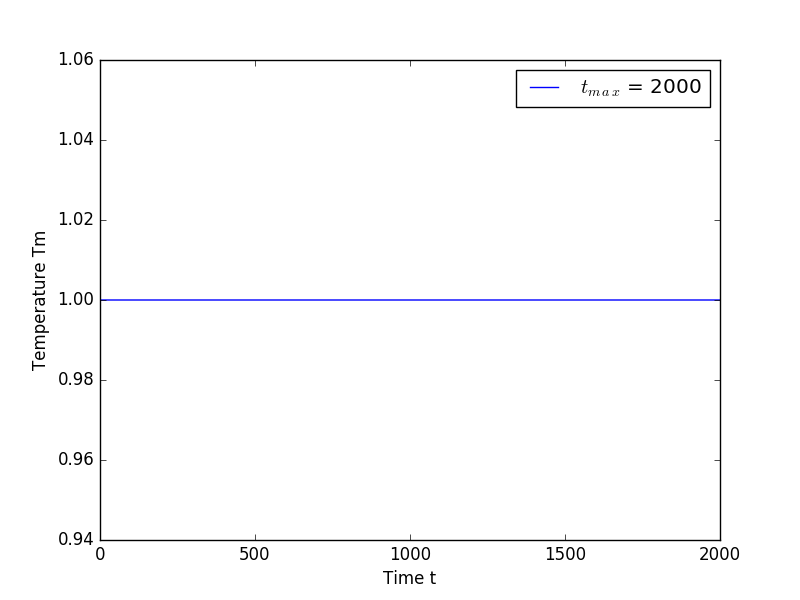
\includegraphics[width=0.7\textwidth]{../dat/berendsen_T1d0_tau3d0_Tm.png}
	\caption{
		Plot of the temperature over time for a desired temperature of $T_\text{des}=1.0$ for a simulation with the Berendsen thermostat and $\tau_T =3.0$.
	}
	\label{berendsenT}
\end{figure}

\begin{figure}[ht]
	\centering
	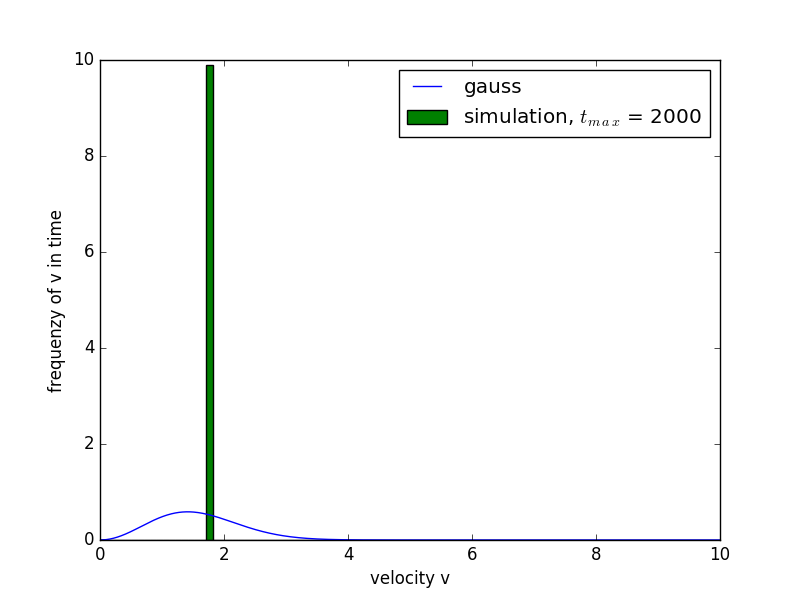
\includegraphics[width=0.7\textwidth]{../dat/berendsen_T1d0_tau3d0_vv.png}
	\caption{
		Plot of the temperature over time for a desired temperature of $T_\text{des}=1.0$ for a simulation with the Berendsen thermostat and $\tau_T =3.0$.
	}
	\label{berendsenvv}
\end{figure}

As you can see the results differ from the further tasks.
The temperature is constant at the desired temperature 1.0. 
There is no fluctuation any more.
It is the same for the velocities. 
The velocity stays constant at a value which gives us the right temperature. 
There is no Gaussian at all.
Of course this will look different for more than one particle with pair interactions, but it would also not fulfill the Gaussian.\\

Because of this the Berendsen thermostat is the worst of the three thermostats (in a physical meaning).

\FloatBarrier